\documentclass[12pt]{beamer}

%%%%%%%%%%%%%%%%%%%%%%%%%%%%%%%%%%%%%%%%%%%%%%%%%%%%%%%%%%
%%%%%%%%%%%%%%%%%%%%%%%%%%%%%%%%%%%%%%%%%%%%%%%%%%%%%%%%%%

\usepackage[orientation=portrait]{beamerposter}
	\usepackage{amsmath, amssymb}
	\usepackage{microtype}
	\usepackage{empheq}
	\usepackage{siunitx}
	\usepackage{dsfont}
	\usepackage{scrextend}
	\usepackage{subcaption}
	\captionsetup{compatibility=false}
	\usepackage{tikz}
	\usetikzlibrary{patterns,arrows,decorations.pathreplacing,hobby}
	\usepackage{graphicx}
	\usepackage{natbib}

	\usepackage{fontspec}
	\changefontsizes{28}
	\setsansfont{Futura}

\usetheme{Berlin}      % or try Darmstadt, Madrid, Warsaw, ...
\usecolortheme{rose} % or try albatross, beaver, crane, ...
\usefonttheme{serif}  % or try serif, structurebold, ...
\setbeamertemplate{navigation symbols}{}
\setbeamertemplate{caption}[numbered]

	\renewcommand{\maketitle}{%
	\begin{center}%
		\Huge\inserttitle\\[5mm]%
		\Large\insertauthor\\[5mm]%
		\Large\insertinstitute%
	\end{center}%
	\vspace*{-1.5ex}%
}

\geometry{
  hmargin=2.5cm, % little modification of margins
}

\setlength{\paperwidth}{24in}
\setlength{\paperheight}{36in}
\setlength{\textwidth}{\paperwidth}
\setlength{\textheight}{0.9\paperheight}
\setbeamersize{text margin left=0.5cm,text margin right=0.5cm}

%beamer definitions

\makeatletter
\definecolor{lightblue}{RGB}{33,140,168}
\definecolor{crimson}{RGB}{218,61,73}
\definecolor{cream}{RGB}{250, 245, 245}
\definecolor{clay}{RGB}{207, 190, 180}

\setbeamercolor{normal text}{fg=black,bg=white}

\setbeamercolor{block body}{fg=black, bg=lightblue!20!white}
\setbeamercolor{block title}{fg=white, bg=lightblue!60!black}


\setbeamercolor{alerted text}{fg=crimson}
\setbeamercolor{item}{fg=crimson}
\setbeamercolor{caption name}{fg=clay!20!black}

\setbeamercolor{example text}{fg=crimson!50!black}
\setbeamercolor{block body example}{fg=black, bg=cream!80!gray} 
\setbeamercolor{block title example}{fg=white, bg=crimson} 

\setbeamercolor{structure}{fg=cream}

\setbeamercolor{background canvas}{bg=cream, parent=normal text}
\setbeamercolor{background}{parent=background canvas}

\setbeamercolor{palette primary}{fg=cream!40!white,bg=crimson!80!black}


	\newcommand*\mystrut[1]{\vrule width0pt height0pt depth#1\relax}
\makeatother

%%%%%%%%%%%%%%%%%%%%%%%%%%%%%%%%%%%%%%%%%%%%%%%%%%%%%%%%%%%
%%%%%%%%%%%%%%%%%%%%%%%%%%%%%%%%%%%%%%%%%%%%%%%%%%%%%%%%%%%

\title{Characterizing Computational Techniques for Experimentally Feasible Non-Local Evolution of Two-Qubit Systems}
\author{Shankar Balasubramanian\hspace{1em} Didi Chang-Park\hspace{1em} Kyle Herndon\hspace{1em} Zane Rossi}
\institute{TJHSST Modern Physics and Optics Lab}
\date{9 June 2015}

\begin{document}
\centering
	\begin{frame}{\maketitle}
	
					   {\bf{Abstract:}} This paper investigates computational methods and presents a computational framework for simulating non-local evolution of two-qubit systems. This evolution may then easily be combined with finite local operations to give control of near-arbitrary precision. Current research has focused on developing the theoretical background which we hope to computationally implement. We will characterize how useful operators (particularly the $CNOT$ gate) are generated in this process, and they will be approximated and performed computationally in optimal time utilizing a adaptive-algorithm approach. We will also analyze the non-local piece of the system Hamiltonian, including determining experimental means of generating it.  Particularly, we will be evaluating its action on the Poincar\'{e}-Bloch-Sphere.

\vfill

		\begin{columns}
			\begin{column}{.45\textwidth}
			
\begin{exampleblock}{Mutation Protocol}
	Mutations are designated on the basis of chance and magnitude. We set a particular threshold value, $\alpha$, which determines whether or not a particular organism's parameters will be mutated. The parameters are the $\beta '$ rotation coefficients which are specified in the exponential form of the local operations. The other changeable parameter, $\mu$, specifies the degree to which the angles will be mutated.
	\begin{figure}[htpb]
		\centering
			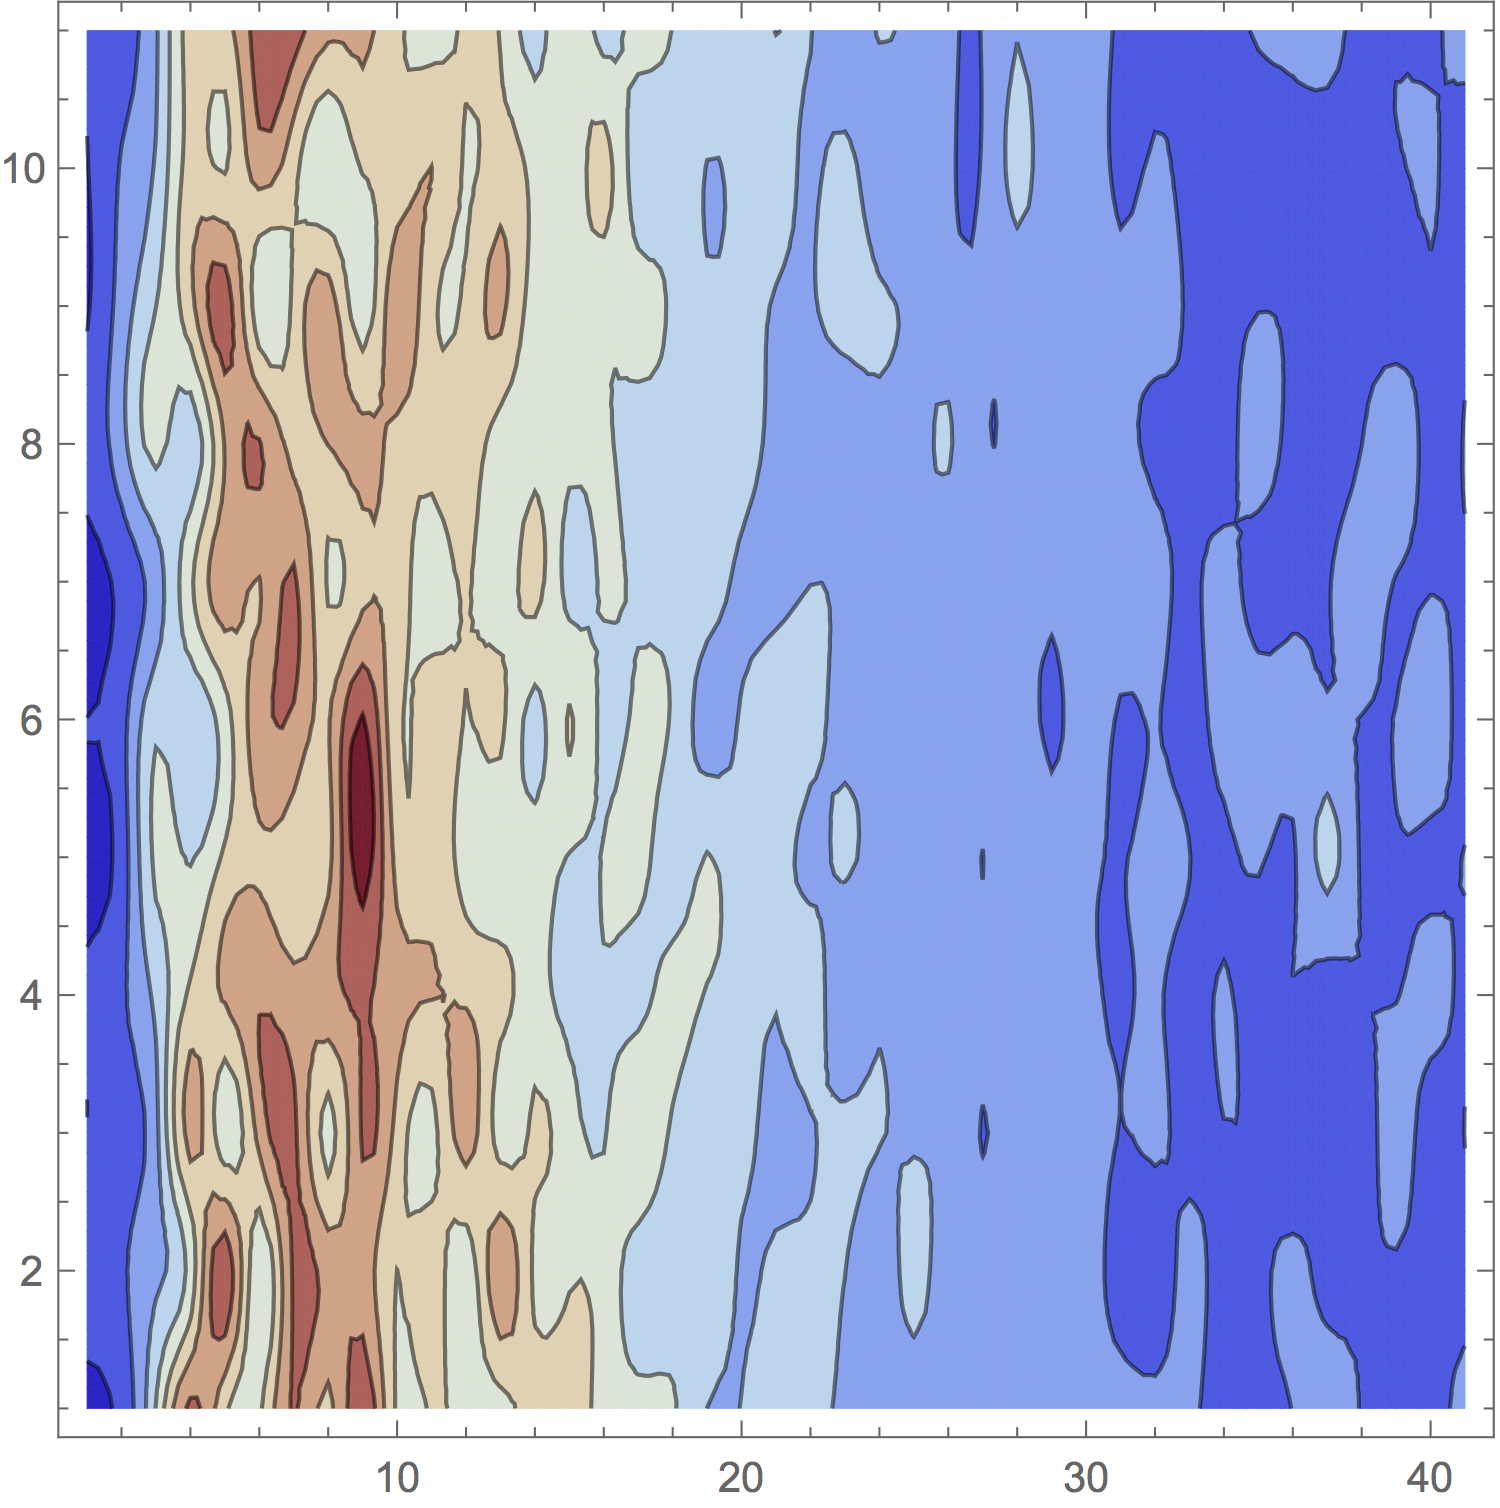
\includegraphics[scale=1.05]{efficiency_plot_col.png}
		\centering
		\caption{This plot shows the fidelity of the best organism in a ten-organism set after $100$ generations with respect to mutation chance and mutation magnitude. The vertical axis, when the value is multiplied by $0.1$, gives the chance in any generation for one of the angles defining an organism to be mutated. The horizontal axis, when multiplied by $0.025$, gives the mutation magnitude (this ranges between $0$ and $1$ radian(s)). The plot shows clear correlation between mutation magnitude and organism success.}
		\label{fig:effplot}
	\end{figure}
	
\end{exampleblock}

\vspace{1em}

\begin{block}{The Space as a Whole}
  A key part to this algorithm's success is knowledge of the search space, and how mobility through it responds to variation in the parameters of its constituent functions. Figure \ref{fig:tot_plot} shows the fidelity, on average, of organisms in the $XX$ problem.

	\begin{figure}[htpb]
		\centering
			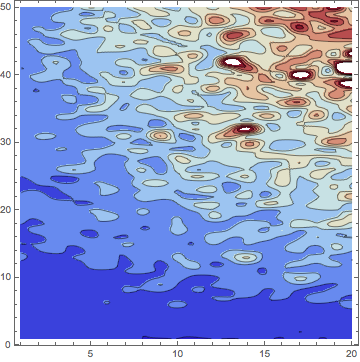
\includegraphics[scale=1.05]{genPlot_50O_20G.png}
		\centering
		\caption{This is a representation of the nature of the search space. Along the horizontal axis is generation number for the set of organisms, and along the vertical is the population of the set. The plot is taken as an average of 20 runs across the entire grid, with the contour plot interpolated between the data at each point; values shown are the fidelity of the best organism on average, and range from 0 to 6.}
		\label{fig:tot_plot}
	\end{figure}
\end{block}
\vspace{1em}
\begin{exampleblock}{Variation in Population and Generation Number}

	\begin{itemize}
	\item Variation in population employs a series of methods used to determine fidelity in a population of a set size, generation number, and gene length. We can then produce a series of partially-evaluated functions that can be mapped over a list of integers. The plotted results of this mapping gives knowledge of a slice of the search space, analogous to partial derivatives, which can help determine which variables produce the best solutions with the smallest computational cost. 
	
	\item Variation in generation number uses the same process, except the slice through the search space is made in a way orthogonal to the original slice. On average, due to the structure of the space, the behavior along one slice is related to that at adjacent slices. 
	\end{itemize}
	\vspace{-1.35em}
\begin{figure}[t!]
    \centering
    \begin{subfigure}[t]{0.5\textwidth}
        \centering
        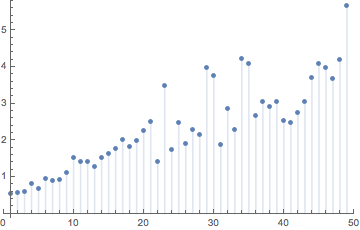
\includegraphics[scale=1.2]{20G_Plot_2.png}
        \caption{A plot of the average of $20$ runs in which the population is along the horizontal axis, and fidelity ($\mathcal{F}$), is along the vertical axis. During these runs, the organism population was brought through $20$ generations, with each organism having two genes.}
        \label{fig:pop_plot}
    \end{subfigure}%
    ~
    \begin{subfigure}[t]{0.5\textwidth}
        \centering
        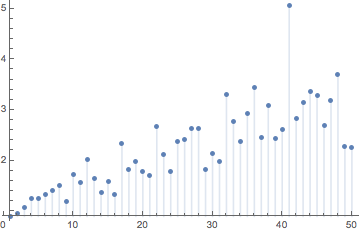
\includegraphics[scale=1.2]{20O_Plot_2.png}
        \caption{A plot of the average of $20$ runs in which the generation number is along the horizontal axis, and fidelity is along the vertical. During this run, the number of generations is taken from $1$ to $50$, while the gene number remains at $2$, and the population is constant at $20$. ($\alpha$ and $\mu$ are preserved from Figure \ref{fig:pop_plot})}
        \label{fig:gen_plot}
    \end{subfigure}

\end{figure}
		\end{exampleblock}


		\end{column}
		
							\begin{column}{.45\textwidth}		

	\begin{block}{The $XX$ Problem} \label{xx}

	This problem represents a proof-of-concept. They purpose of this scheme is to generate complex unitary evolution operators, and not only is the problem

	\begin{empheq}[box=\fbox]{align}
		\mystrut{1em} exp\{\sigma_x \otimes \sigma_x\} \mapsto exp\{\sigma_x \otimes \sigma_x\}
	\end{empheq}

	attempting to represent a simple unitary evolution operator, it is attempting to represent the one we began with! Ideally, the results of a high-fidelity simulation in this case would yield identity matrices which produces the same result with two genes. To demonstrate trends in efficiency, we have produced a small table of fidelities, for example. 

	\begin{table}[htpb]
		\centering
			\begin{tabular}{||l | l l ||} 
			\hline
				Pop. & 20 Gen. & 50 Gen. \\ [0.5ex] 
			\hline
				10  & 0.63   & 0.95      \\ 
				25  & 0.86   & 1.71      \\
				50  & 1.17   & 2.17      \\
				100 & 4.79   & 2.31      \\
			\hline
			\end{tabular}
		\centering
		\caption{A chart of fidelities for the $XX$ problem. These values are not averaged, and give some feel as to the variations inherent to each trial.}
	\end{table}

	Apart from fidelity, the optimal organisms themselves may be analyzed. The algorithm, at the end of its search, provides the organism with the largest fidelity. This organism is represented by two lists, each containing the set of $A_i$ or $B_i$ in terms of three angles. These lists are then transformed back into traditional matrices, and combined to compare with the goal unitary operator. In a two-gene, 100 organism, 20 generation simulation, we can see that the generated matrix is very close to the predicted identity. 

	\begin{equation}
	A_1\otimes B_1 = 
	\begin{pmatrix}
		{\color{crimson}\mathbf{0.99}}  &  0.08  &  0.01  &  0.00\\
		0.04  &  {\color{crimson}\mathbf{0.99}}  &  0.00  &  0.01\\
		0.01  &  0.00  &  {\color{crimson}\mathbf{0.99}}  &  0.08\\
		0.00  &  0.01  &  0.04  &  {\color{crimson}\mathbf{0.99}}
	\end{pmatrix}
	\end{equation}

	This simulation produced solid results because there exists a perfect solution that is easily predicted. There is no guarantee that, given a particular number of genes, a goal operator can be perfectly simulated \cite{victer}, only that more genes allows \emph{better} simulation. We expect to converge to more exotic goal operators slowly in comparison.
\end{block}
\vspace{1em}

\begin{exampleblock}{The $XY$ Problem}

	In the interest of a less trivial problem, we attempt to move to another simple represented Hamiltonian ($\sigma_y \otimes \sigma_y$). We can represent this concisely by

	\begin{empheq}[box=\fbox]{align}
		\mystrut{1em} exp\{\sigma_x \otimes \sigma_x\} \mapsto exp\{\sigma_y \otimes \sigma_y\}
	\end{empheq}

	The fidelities can be charted as done in the previous problem, or we may produce a larger chart of the space as in Figure \ref{fig:tot_plot}. 

	\begin{figure}[htpb]
		\centering
			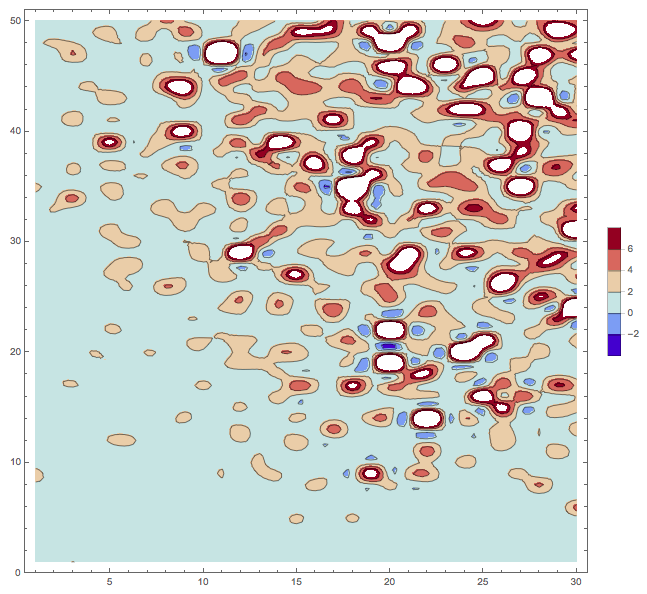
\includegraphics[scale=0.6]{xyPlot_50O_20G.png}
		\centering
		\caption{This shows the same plot as Figure \ref{fig:tot_plot}, but in the context of the $XY$ problem. A scale is included to show the fidelities. Note the absence of well defined contours.}
		\label{fig:xy_plot}
	\end{figure}    
    As mentioned previously, we can also look at the operators generated from the best organism's set of angles (i.e. $A_1 \otimes B_1$ and $A_2 \otimes B_2$). Even general trends in these can be helpful in recognizing traits of solutions.
    \begin{figure}[htpb]
		\centering
			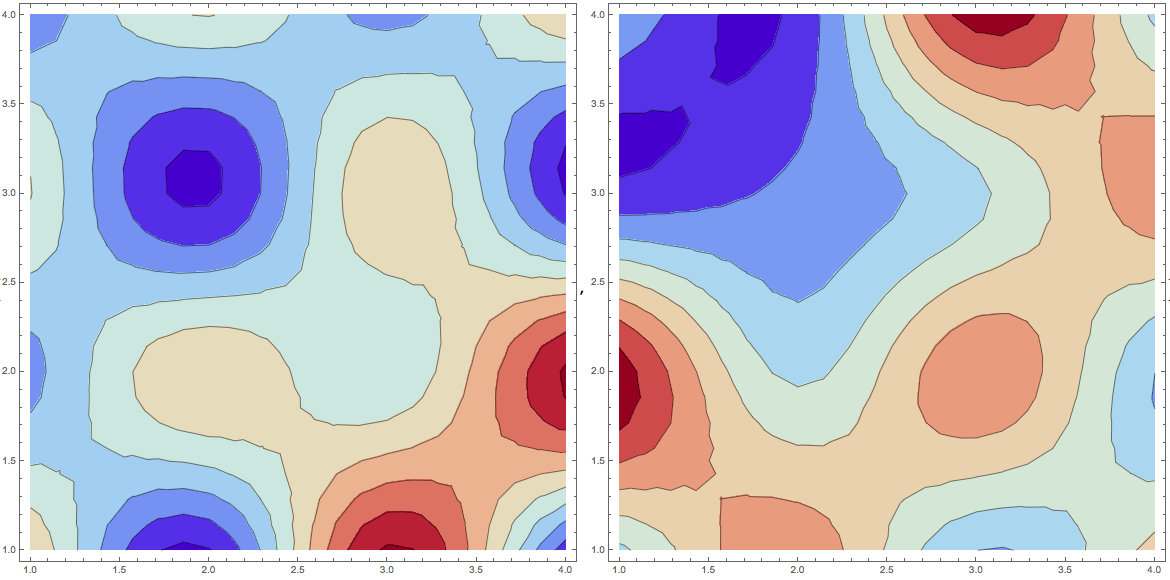
\includegraphics[scale=0.5]{xy_test_matrices.png}
		\centering
		\caption{A contour plot of the local operations ($A_i \otimes B_i$) performed by an organism in the $XY$ problem. Note that this is an interpolation of a matrix's elements (a four by four grid) and is therefore a useful heuristic, rather than a concrete tool for analysis. The modulus value of the entries were taken, and thus phase factors are lost.}
		\label{fig:xy_matrix}
	\end{figure}

	In these types of problems, high fidelities can be reached, but the algorithm is less stable, and generally requires a larger population to produce similar quality. 
	\end{exampleblock}


	%	%%%%%%%%%%%%%%%%%%%%%%%%%%%%%%%%%%%%%%%%%%%%%%%%%%%%%%%
%

%
%	%%%%%%%%%%%%%%%%%%%%%%%%%%%%%%%%%%%%%%%%%%%%%%%%%%%%%%%

		\end{column}
	

	
		\end{columns}
	\end{frame}

%%%%%%%%%%%%%%%%%%%%%%%%%%%%%%%%%%%
%% Half slides %%%%%%%%%%%%%%%%%%%%%%%%%%%	
	\begin{frame}
		\begin{columns}
			\begin{column}{.45\textwidth}
				\begin{block}{Background}
					The ultimate goal of Control Theory is the ability to arbitrarily manipulate the state of an ensemble of qubits. In the context of quantum computation, this problem is reduced further: basic quantum gates allow for modular systems \cite{bremner}. However, the generation of these gates is non-trivial, and the arbitrary Hamiltonian is, in general, not readily constructible. Often one will wish to achieve a specific unitary evolution operator or gate $U$ corresponding to the solitary time evolution of a Hamiltonian $H$. When $H$ may not be engineered easily, the evolution can be achieved in other ways \cite{bremner} , often involving the use of local operations (LO), repeated measurements on the system \cite{bennett}, along with standard Hamiltonian-driven evolution drawing from some collection (possibly a one element collection) $H_1, H_2, \cdots, H_n$, all of which \emph{can} be lucratively generated.

	In the simplest case, a two particle system, the Hamiltonians involved may contain non-local terms, usually corresponding to particle-particle interactions. This paper will propose a framework for taking the general non-local Hamiltonian \cite{bennett} 
	\begin{equation}
	H = A \otimes \mathds{1} + \mathds{1} \otimes B + \sum_{ij} M_{ij}\,  \sigma_i \otimes \sigma_j
	\end{equation}
	and interspersing its non-local part's evolution with LO to achieve a desired $U$. It is only the non-local part of the Hamiltonian which must be studied, and through decomposition of this piece into its canonical form, and some insight into Lie Theory, we are able to formulate a computational approach \cite{haselgrove}. Devising a scheme to generate a $U$ from a collection of available operators and Hamiltonians has direct applicablity to a variety of problems, but cannot be done purely analytically on a massive scale, thus making a computational method necessary.
				\end{block}
				\vspace{1em}
				\begin{exampleblock}{Adaptive Algorithm Theory}
	Adaptive algorithms attempt to mimic the process of evolution by the mechanisms of mutation and natural selection. A set of mathematical objects dubbed \emph{organisms}, each containing some set of data, are subjected to tests against some metric depending on the organism's features \cite{weise}. This is considered one \emph{generation}, and the best organisms of each generation are bred together (by some deterministic algorithm) and mutated to compete in the next generation. In preparation for performing a process like the one described, we take three major steps.
	\begin{itemize}
	\item To begin, the degrees of freedom of the system should be analyzed, as these will function as the dimensions of the search space. During this process, the degrees which are less pertinent to a solution's fidelity should be identified and their relative mutation amplitude and frequency altered accordingly.

	\item Next, the mutations assigned to each degree of freedom will be designed so as to best approach a (hopefully) global extrema in the search space. In general, more volatile mutations will be given to the more effective degrees of freedom, and all mutations will decrease in magnitude and frequency as the number of generations increases \cite{satsangi}

	\item Finally, we need determine the method by which the best organisms of each generation are bred (combined in a way that may retain traits of both.). Note that there is no guarantee under any binary operation that the resulting object will have the same advantages assigned to the parent objects. In the case of well-defined and relatively smooth systems, this breeding will often resemble a sort of average, and the child will often perform similarly to the parents. 
	\end{itemize}
	With these in mind, we can visualize the process as a sort of traversal of a complex multidimensional search space.
\begin{figure}[htpb]
	\centering
	\begin{tikzpicture}[scale=1.8, use Hobby shortcut]

	% main bounding shape
	\draw[ultra thick, closed=true, dash pattern=on 6pt off 6pt] (2.5,4.5) .. (3.3,6.5) .. (5,7.5).. (7.5,7.9).. (10,7.5).. (11,6.5).. (11,4.5) ..(8.5,2).. (6,3.5).. (3,2).. (2.5,4.5);

	%interior grid
	\begin{scope}
		\clip[closed=true] (2.5,4.5) .. (3.3,6.5) .. (5,7.5).. (7.5,7.9).. (10,7.5).. (11,6.5).. (11,4.5) ..(8.5,2).. (6,3.5).. (3,2).. (2.5,4.5);

		\draw[step=1,gray,thick] (0,0) grid (15,15);
	\end{scope}

	% organism paths
	\draw[ultra thick, color=lightblue] (4.5, 4.5) -- (6.5, 4.5);
	\draw[ultra thick, color=crimson, dash pattern=on 0.2cm off 0.2cm] (4.5, 4.5) -- (6.5, 4.5);
	% yeah, that's right, I just did that (dashed overlay)
	\draw[ultra thick, -latex, color=lightblue] (6.5, 4.5) -- (7.5,4.5) -- (7.5,3.5) -- (8.5,3.5) -- (8.5,7.5);
	\draw[ultra thick, -latex, color=crimson] (6.5, 4.5) -- (6.5,6.5);

	% organism circle
	\fill[fill=lightblue] (4.5,4.5) circle (0.4cm);

	% organism symbol and arguments
	\node[right] at (-0.5, 9) {\large{$\Theta:\;$ \small{\sc{Arguments}}}};
	\draw (-0.5, 8.5) -- (4, 8.5);

	\node[right] at (-0.5, 6) {$\{A_i\}\;\;\{B_i\}$};
	\node[right] at (-0.5, 5) {$\{t_i\}\;\;$};
	\node[right] at (-0.5, 8) {$H:\;$ \small{\sc{Constant}}};
	\node[right] at (-0.5, 7) {$N:\;$ \small{\sc{Constant}}};

	\end{tikzpicture}
	\centering
		\caption{
		This is a simplification; the organism being tested is represented by the circle in blue, while the search-space (which has a defined metric represented by the grid) surround it. The paths of different color shown represent the non-deterministic paths possible as the organism mutates and is bred with other successful organisms. The actual space being searched is not two- but many-dimensional.
		}
	\end{figure} 
\end{exampleblock}
				\vspace{1em}
	\begin{block}{Group Theory Exploitation}

	The entirety of this simulation scheme is done with the pauli basis, and this allows their wonderful properties to be exploited. Given further research, the algorithm would implement group theory concepts in its heuristic, but currently, this idea is only used in data compression, and the breeding/mutation of matrices.
	
	The local operations described in the preceding section can be realized as unitary matrices, and described by three angles. Because of this, we can imagine all possible unitary operators as lying on the surface of the 3-Sphere\cite{aerts}.
		\begin{figure}[htpb]
		\centering

		\begin{tikzpicture}[use Hobby shortcut, thick, scale=2]
		
		\tikzset{
		    partial ellipse/.style args={####1:####2:####3}{
        		insert path={+ (####1:####3) arc (####1:####2:####3)}
    		}
		}

		% clipping for ellipse

		\begin{scope}
			\clip (0,0) circle (3cm);
			\clip (-4,0) rectangle (4,-4);

			\fill[lightblue] (0,0) circle (3cm);
		\end{scope}

		% ellipse drawn
		\draw[ultra thick, lightblue!80!black] (0,0) ellipse (3cm and 1cm);

		\fill[lightblue] (0,0) ellipse (3cm and 1cm);

		\fill[lightblue!60!white] (0,0) ellipse (2cm and 0.66cm);

		\fill[lightblue!20!white] (0,0) ellipse (1cm and 0.33cm);

		% markings and text

		\draw[ultra thick] (0,0) circle (3cm);

		\draw[ultra thick, crimson, -latex] (0,0) [partial ellipse=0:-120:3.5cm and 1.33cm];
		\draw[ultra thick, crimson, -latex] (0,0) [partial ellipse=180:120:3.5cm and 3.5cm];
		\fill[crimson] (0,0) ellipse (0.3cm and 0.1cm);
		\draw[ultra thick, crimson, -latex'] (-0.1,0) -- (-2.9, 0);

		\end{tikzpicture}
		\centering
		\caption{A pictorial representation of the 3-sphere: the upper half has been removed for clarity. The three arrows represent the degrees of freedom along the 3-sphere's surface, the points of which have been projected to the interior of a 2-sphere. (The arrow along the traditional `radius', if extended, gives degeneracy). Despite implication there is no preferred direction along which to move across the 3-sphere.}
	\end{figure}


\end{block}

%%%%%%%%%%%%%%%%%%%___ COMPUTE ___%%%%%%%%%%%%%%%%
%%%%%%%%%%%%%%%%%%%%%%%%%%%%%%%%%%%%%%%%%%%%%%%%%%

					\end{column}
			
			\begin{column}{.45\textwidth}

	
	%%%%%%%%%%%%%%%%%%%%%%%%%%%%%%%%%%%%%%%%%%%%%%%%%%%%%%
			\begin{exampleblock}{The $CNOT$ Problem}

	\begin{empheq}[box=\fbox]{align}
		\mystrut{1em} exp\{\sigma_x \otimes \sigma_x\} \mapsto CNOT
	\end{empheq}

	The purpose of this simulation scheme is to generate methods to create useful quantum operators. These manifest in the canonical quantum gates. Among the most notorious of these (and from which all others can be constructed \cite{oliviera}) is the $CNOT$ gate, represented in matrix form as such

	\begin{equation}
	CNOT = 
	\begin{pmatrix}
		1  &  0  &  0  &  0  \\
		0  &  1  &  0  &  0  \\
		0  &  0  &  0  &  1  \\
		0  &  0  &  1  &  0 
	\end{pmatrix}
	\end{equation}

	This operator allows one qubit's state to affect the operation applied to another. This is incredibly pertinent in control theory. By the nature of the correlation it implies between particles, this operator is not the tensor product of two local operators. Due to this, the non-local piece of the initial Hamiltonian must take the brunt of the work in producing $CNOT$. 

	Initial runs yield exotic matrix plots 
	
	\begin{figure}[htpb]
		\centering
			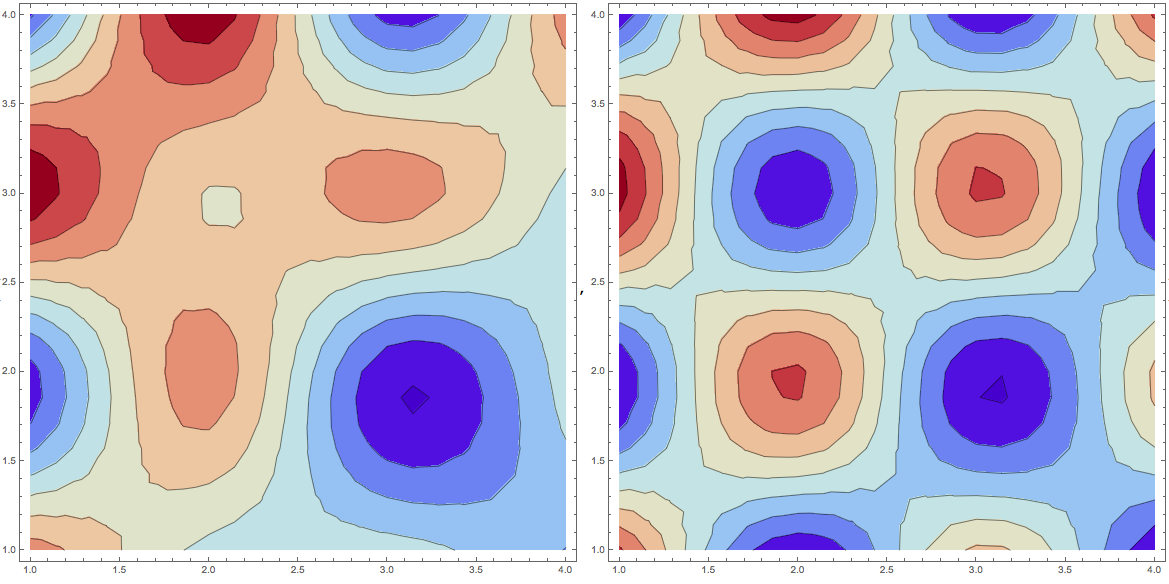
\includegraphics[scale=0.4]{cnot_matrices.png}
		\centering
		\caption{Plots of the LO for the $CNOT$ problem. Note that the operators are markedly different, but maintain a concentration of value in the upper off-diagonals.}
		\label{fig:cnot_matrix}
	\end{figure}

	However, the difficulty of simulating this operator manifests itself in relatively low fidelities given the same generation and population numbers used in the previous problems. There are a few possible ways to increase fidelity (or rather, the potential fidelity) of $CNOT$ simulations.
     \end{exampleblock}
     \vspace{1em}

			\begin{block}{The 0 Problem}

	Although there are many simulations possible that are useful to control theory, the final example will be in the simulation of the zero-Hamiltonian, or the stasis of a system. Engineering dynamic Hamiltonians has distinct uses, but preserving the state of the system is unique in two respects: it represents the negation of the original Hamiltonian, and it allows the state of a system to be preserved indefinitely. The problem is represented as such (the zero-Hamiltonian produces the identity as its unitary evolution operator). 

	\begin{empheq}[box=\fbox]{align} \label{identity}
		\mystrut{1em} exp\{\sigma_x \otimes \sigma_x\} \mapsto \mathds{1}
	\end{empheq}

	To give a feel for the fidelity, below is a sampled unitary evolution operator approximation from an average run at 100 organisms and 20 generations. 

	\begin{equation}
	\tilde{U} = 
	\begin{pmatrix}
		{\color{crimson}\mathbf{0.86}}   &  0.07  &  0.07  &  0.10  \\
		0.07  &  {\color{crimson}\mathbf{0.86}}   &  0.09  &  0.07  \\
		0.17  &  0.10  &  {\color{crimson}\mathbf{1.08}}   &  0.15  \\
		0.10  &  0.17  &  0.14  &  {\color{crimson}\mathbf{1.08}}  
	\end{pmatrix}
	\end{equation}

	\end{block}
				\vspace{1em}
								\begin{exampleblock}{Conclusion}
We have identified various aspects of using adaptive algorithms that are beneficial and detrimental in determining local operation sets to simulate an arbitrary gate. 
	\begin{itemize}
\item Although our results have consistently agreed mathematically, with fairly large fidelity, the run-time grows linearly with the number of organisms, generations, and gene number. This can only be countered well by running this program with multiple processors (i.e. in parallel, for which this algorithm is well-suited) \cite{umbarkar}.
\item Moreover, much of the computation time derives from matrix multiplication, which is a daunting task to optimize. Perhaps, using a more effective algorithm will improve the run-time efficiency of the code as well. We can however partially ease matrix multiplication by taking advantage of particular expansions of matrix exponentials, which can be truncated depending upon our desired accuracy.
\item Using commutation relations and Lie algebras may immensely help with the reduction of run-time as well (this involves both engineering the heuristic and the initial populations). The methods forming the basis of this scheme are naive, and base little of their workings off of the defining tricks of linear algebra and group theory. There are properties to be exploited, but we chose to produce a functional process before an optimal one. We also wish to design better ways of representing the resulting operators, to give more intuition about their structure. %The last sentence doesn't quite fit
\end{itemize}
Although we compromise time for fidelity, our efforts in implementing adaptive algorithms to solve this quantum computation problem has yielded success in producing a viable solution sets. With complex systems, as are necessary to produce non-trivial quantum computations, analytical methods for generating the correct unitary evolution operator are simply not feasible. With the proper improvements, non-deterministic methods such as the one here could prove useful in the development of quantum computation. 


					
				\end{exampleblock}
				\vspace{1em}
				
				\begin{block}{References}
				\changefontsizes{21}

					\bibliographystyle{plain}
				\bibliography{ref}		
				\end{block}
			\end{column}	
		\end{columns}
	\end{frame}	
\centering


\end{document}